% \chapter{Perturbative Approach in Strong Lensing}
\section{Basic Ideas}

{\bf \Large We'll give some intro comments first, a modified version of these:}

The SLPM lets us analyze images without assuming a model.

Much faster for forward simlns.

Nice analytic formulae for lens curves and arcs.

Works well in many regimes.

And some part of this:

Let us assume that the two-dimensional projected density $\Sigma$ of a
strong gravitational lens system is axially symmetric and centered at
the origin. Let us assume that the lens is dense enough to reach
critical density at a given radius $\re$. Under such an hypothesis,
the image of a point source placed in the source plane at the origin
will be a perfect ring at $\re$. However, if the source is not
perfectly at the center, or the potential is not perfectly
axisymmetric, the perfect ring is broken into arcs.

To investigate this fact, we will use the lens equation $\vec{r}_s =
\vec{r} - \vec{\alpha}$, where $\vec{r}_s$ is the angular position of
the point source in the source plane (see fig. in Narayan and
Bartelmann for this [get proper ref for this fig]), $\vec{r} = r
\hat{r} $ is the angular position of the point source in the image
plane, and $\vec{\alpha}$ is the deflection angle, which is equal to
the radial gradient of the 2D projected potential $\phi$...

...

Note that now the perturbed distance $x$ is in the image plane.

To recap: $r_s, y$ are in the source plane, while $r, x$ are in the image plane.

Now we do a Taylor series expansion of the potential:

\beq
\phi = \phi_0 + \eps \psi = \sum_{n=0}^\infty {1 \over n!} \left. {d^n \phi_0 \over dr^n }\right|_{\re} (r-\re)^n + \eps {1 \over n!} \left. {d^n \psi(\theta) \over dr^n }\right|_{\re} (r-\re)^n
\eeq

or

\beq
\label{eq:tse}
\phi  = \sum_{n=0}^\infty \left[ {1 \over n!} \left. {d^n \phi_0 \over dr^n }\right|_{\re} + \eps {1 \over n!} \left. {d^n \psi(\theta) \over dr^n }\right|_{\re} \right] (r-\re)^n
\eeq

And now define

\beq
C_n \equiv {1 \over n!} \left. {d^n \phi_0 \over dr^n }\right|_{\re}
\eeq

\beq
f_n(\theta) \equiv  {1 \over n!} \left. {d^n \psi(\theta) \over dr^n }\right|_{\re}
\eeq

So that we can write  eq.(\ref{eq:tse}) as

\beq
\label{eq:tse2}
\phi  = \sum_{n=0}^\infty \left[ C_n + \eps f_n  \right] (r-\re)^n
\eeq

where $f_n = f_n(\theta)$.


Now let's go back and substitute eq.~\eqref{eq:rspert}) and eq.~\eqref{eq:rpert}) into eq.~\eqref{eq:rs}) to find
\beq
\eps y = \left( \re + \eps x -  {\prtl  \phi \over \prtl r} \right) \hat{r} - {1 \over \re + \eps x}  {\prtl  \phi \over \prtl \theta} \hat{\theta}
\eeq

More steps, then:


\beq
\label{eq:rsexpanded}
 y = \left[ \kt x - f_1 \right] \hat{r} - {1 \over \re} {\prtl f_0 \over \prtl \te}  \hat{\theta}
\eeq

which is Alard eq.8 (remember he set $\re \equiv 1$).

Should we put the actual technical steps in an appendix, since Alard skips so many..?


\subsection{Critical Curves and Caustic Lines in the Perturbative Approach}

{\bf \Large Can shorten, get a modified version of this:}

We will now obtain the equations of the critical curves in the lens
plane (corresponding to the caustic curves in the source plane).

First write eq.~\eqref{eq:rsexpanded} in Cartesian coordinates (expanding
the unit polar vectors, eq.~\eqref{eq:unitvs}, and taking
$\vec{y}=(y_1,y_2)$ in the source plane and $\vec{r}=(r,\te)$ in the
lens plane:
%Note that as we have not considered the position of the source,
%we have $\bar{f}_i=f_i$ and therefore
\begin{eqnarray}
y_{1} &=& [\kt x - f_1]\cos{\te}+\frac{1}{\re}\frac{d f_0}{d\te}\sin{\te} \label{y_1}\\
y_{2} &=& [\kt x - f_1]\sin{\te}-\frac{1}{\re}\frac{d f_0}{d\te}\sin{\te} \label{y_2},
\end{eqnarray}

The Jacobian of the transformation from polar to Cartesian coordinates is given by

\begin{equation}
J=\frac{\prtl y_1}{\prtl r}\frac{\prtl y_2}{\prtl \te}-\frac{\prtl y_1}{\prtl \te}\frac{\prtl y_2}{\prtl r}.
\label{jacob}
\end{equation}

The critical lines are defined by the condition $J=0$. This leads after some work to the expression for the tangential critical curve:

\begin{equation}
x=\frac{1}{\kt}\left[f_1+\frac{1}{\re}\frac{d^2f_0}{d\te^2}\right] \label{xte}.
\end{equation}


Or in parametric form as \beq
\vec{r}_{\mathrm{crit}}= \left[(\re
  +x)\cos{\te},(\re+x)\sin{\te}\right],\quad 0 \leq \te < 2\pi.  \eeq


And for the parametric equation for the tangential
caustic:

\begin{eqnarray}
y_{1_\mathrm{caust}} &=& \frac{1}{\re}\frac{d^2f_0}{d\te^2}\cos{\te}+\frac{1}{\re}\frac{df_0}{d\te}\sin{\te}\\
y_{2_\mathrm{caust}} &=& \frac{1}{\re}\frac{d^2f_0}{d\te^2}\sin{\te}-\frac{1}{\re}\frac{df_0}{d\te}\cos{\te}
\end{eqnarray}



%%%%%%%%%%%%%%%%%%%%%%%%%%%%%%%%%  From before

Getting Alard eq.33 from 31 is straight, and from there we may obtain
% I (MSSG) got most of the way to 
A.eq.34 from 33 and 32.
% with some small hiccups..

\subsection{Reconstruction of Images}

One advantage of the perturbative approach is that it allows us to
construct the lensed images from sources located near the
tangential caustic.  In this section we study the mapping of 
circular and elliptical contours using this formalism.

\subsection{Circular Sources}

\begin{figure*}{r}
  \begin{center}
%  \centering{\epsfig{Fig_subsstructure.eps,width=0.45\textwidth}}
   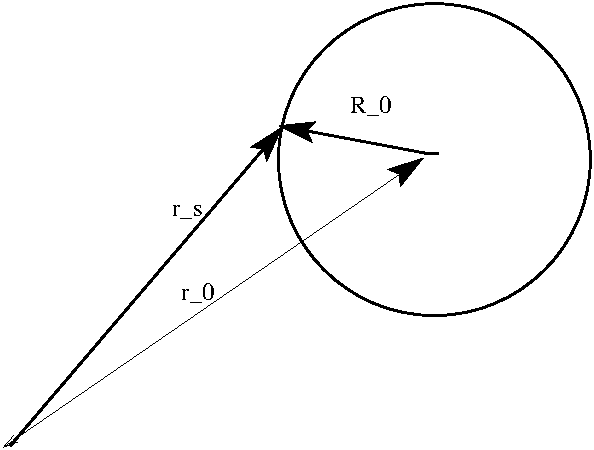
\includegraphics[width=0.35\textwidth]{graphics/sourceplane.pdf}
  \end{center}
    \caption{\label{fig:circular_source}Circular source geometry in the source plane.}
\end{figure*}

Notation: $ \vec{r}_{0}$ points from the origin (i.e center of the
source plane, which is the point we see looking directly on-axis from
us through the lens to the source) to the center of the actual source
object (which might be e.g a small face-on spiral galaxy), $
\vec{R}_{0}$ is the vectorial radius of this source from its center,
and $ \vec{r}_{s}$ is the vector from the origin to some point on the
edge of the circular source. See Fig.~\ref{fig:circular_source} for this
configuration.


...

Solving this for $x(\te)$, the radius of the arc in the image plane as
a function of theta, the following two solutions are obtained, the
negative and positive solutions corresponding to the inner and outer
edges of the arc.:

\beq
\label{eq:xsoln}
x = \frac{1}{\kappa_2}\left[ \overline{f}_{1}(\theta) \pm \sqrt{R_0^2 - \left( \frac{1}{\re}\frac{\partial \overline{f}_0(\theta)}{\partial \theta} \right)^2} \right]. \;\;\;
\eeq



Thus, given the source radius $R_{0}$ and position $(x_0,y_0)$ we can
draw the arcs using eq.~\eqref{eq:xsoln}). The parametric equation for the
arcs images is given by

\beq
\vec{r}= \left[(\re +x)\cos{\te},(\re+x)\sin{\te}\right], \quad 0 \leq \te < 2\pi.
\eeq


\subsubsection{Elliptical Source Contours with Aligned Axes}
%%%%%%%%%%%%%%%%%%% Gabriel
% {\bf If someone have doubts about this procedure, let me know \ldots}

We now extend the discussion of the previous section to elliptical contours.

It is straightforward to verify:

\beq
\bar{y}_{1s}=\dfrac{\eta_s\cos{(2\te)}}{S}\bar{y}_{2s}\pm \frac{1}{S}\sqrt{S R_0^2-(1-\eta_s)\bar{y}^2_{2s}}
\eeq

where $S=1-\eta_s\cos{(2\te)}$. Substituting eq.~\eqref{bar_y1} and eq.~\eqref{bar_y2} into the equation above, we obtain

\beq
x = \frac{1}{\kappa_2} \left\{\bar{f}_{1}(\theta) + \frac{\eta_s\sin(2\theta)}{S}\left(\frac{1}{\re}\dfrac{\partial \bar{f}_0(\theta)}{\partial \theta}\right) \pm \frac{1}{S}\sqrt{SR_{0}^2 - (1-\eta_s^2)\left[ \frac{1}{\re}\frac{\partial \bar{f}_0(\theta)}{\partial \theta}\right]^2}  \right\}.
\label{elliptical_contour}
\eeq

The parametric equation now for the images of elliptical sources of this form is

\beq
\vec{r}= \left[(\re +x)\cos{\te},(\re+x)\sin{\te}\right], \quad 0 \leq \te < 2\pi.
\eeq


\subsection{Elliptical Source Contours in the General Case (Nonaligned Axes)}

In the general case, when the source is not aligned to the semimajor axis of the potential, the vectorial equation of an elliptical contour is

\beq
\label{eq:ellipsetheta}
\vec{R}_0=\left(\sqrt{1-\eta_s} \, y^\prime_{1s},\sqrt{1+\eta_s} \, y^\prime_{2s}\right)
\eeq
where the source is oriented at an angle
$\te_0$ \wrt\ the  semimajor axis,  and $y^\prime_{is}\, (i=1,2)$ are obtained by rotating the coordinate system of the source by an angle $\te_0$,
i.e
\begin{equation}
\left(\begin{array}{c}y^\prime_{1s} \\ y^\prime_{2s} \end{array}\right)=\left[\begin{array}{c c}%
\cos{\te_0} & \sin{\te_0}\\ -\sin{\te_0} & \cos{\te_0} \end{array} \right]\left( \begin{array}{c} y_{1s}\\ y_{2s}\end{array}\right)
\end{equation}

Using eqs.~(\ref{y_1s}-\ref{bar_y2}) it is straightforward to verify
\bea
y^\prime_{1s}&=&\bar{y}_1\cos{\tilde{\te}}+\bar{y}_2\sin{\tilde{\te}}\\
y^\prime_{2s}&=&\bar{y}_1\sin{\tilde{\te}}-\bar{y}_2\cos{\tilde{\te}}\\
\tilde{\te}&\equiv&\te-\te_0
\eea

Now, following the procedure shown above, is straightforward to obtain the expression for the images coming from
lensed elliptical sources (with orientation $\te_0$).  It is given by the Eq.(\ref{elliptical_contour}) with $\te$ replaced by $\tilde{\te}$, i.e.

\bea
x &=& \frac{1}{\kappa_2} \left\{\bar{f}_{1}(\theta) +%
\frac{\eta_s\sin(2\tilde{\theta})}{S}\left(\frac{1}{\re}\dfrac{\partial%
\bar{f}_0(\theta)}{\partial \theta}\right) \pm \frac{1}{S}\sqrt{SR_{0}^2 -%
(1-\eta_s^2)\left[ \frac{1}{\re}\frac{\partial \bar{f}_0(\theta)}{\partial
\theta}\right]^2}  \right\}.\label{elliptical_contour2}\\
S&\equiv& 1-\eta_s\cos{(2\tilde{\te})}\nonumber
\eea
This is the eq.~(28) of Peirani et al. 2008 (recall again, they set $\re=1$ and $\eta_s=\sqrt{2\eta_0}$)

%\beq
%\label{eq:ellipse}
%(1-\eta_s)x_s^2 + (1+\eta_s)y_s^2 = R_{0}^2.\;\;\;
%\eeq

As we can see, the condition for the formation of images is given by
\begin{equation*}
S\,R^2_0>(1-\eta^2_s)\left[\frac{1}{\re}\dfrac{\prtl \bar{f}_0}{\prtl \te}\right]^2
\end{equation*}

And therefore, the number of images is given by the quantity of times over $\theta = 0 $ to $2 \pi$ that the expression of the radicand in eq.~\eqref{elliptical_contour2} switches sign, divided by two.


\section{Measurements of the arc properties}

One of the great advantages of the Perturbative Method is that it
allows us to calculate the analytical expressions for the images contours
coming from lensed sources.

\begin{figure*}[!htp]
\resizebox{\hsize}{!}{
\subfigure{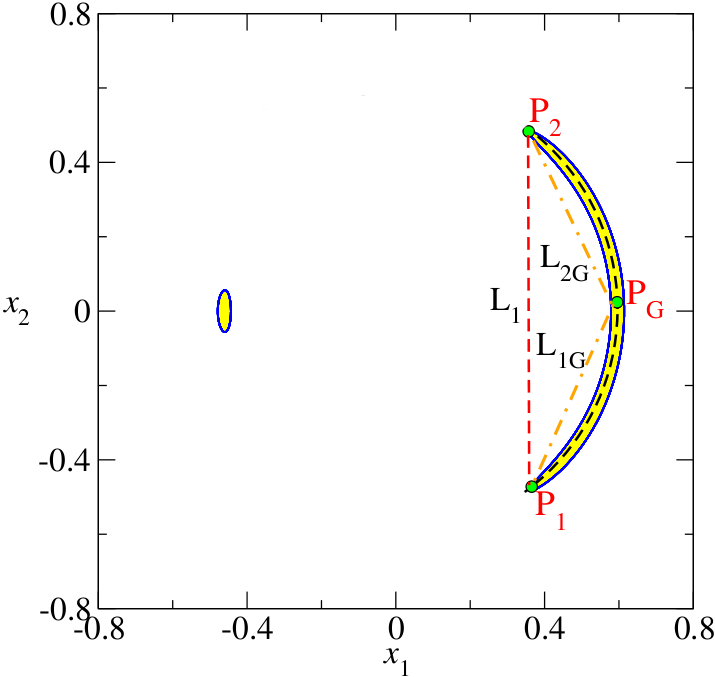
\includegraphics{graphics/measure_arc2.png}}
\hspace{3.cm}
\subfigure{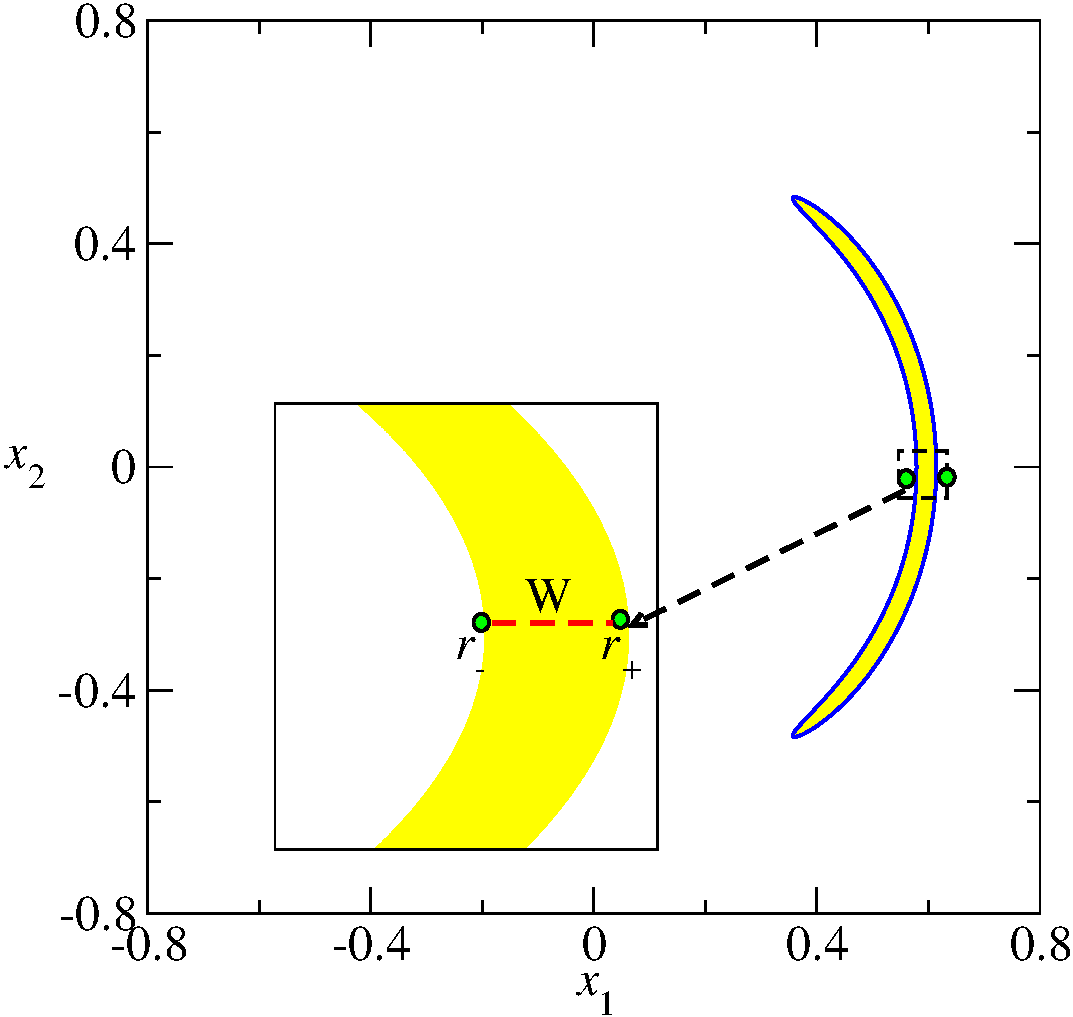
\includegraphics{graphics/measure_arc_w.pdf}}}
\caption{\label{measure_arcs} Method used to measure the length
and width of the images. Left Panel: Schematic representation for the
measurement of the length. Right Panel: Schematic representation for the
measurement of the width}
\end{figure*}


Following Pedro's ideas, shown in his Master Degree Thesis {We need to
  start building a bibliography}, we will give the expressions for the
measurements of the Length, Width and area of the
arc-images. Basically, Pedro shows three methods for measuring the
length of the arcs, denoted $L_1$, $L_2$ and $L_3$, and two methods
for measure the width of the arcs, denoted $W$ and $W_q$.  The first
method is overly simplistic and will not be considered in this report,
except to introduce the geometry of the arcs. We will adapt the second
and third methods in the framework of the Perturbative Method and also
to propose a method similar to Clecio's Method to measure the length.


In the Perturbative Method, the inner and outer radial vector of an arc
are given by

\bea
\vec{r}_{+}&=&(\re + x_{+})\cos{\te}\hat{\imath}+(\re
+x_{+})\sin{\te}\hat{\jmath}\label{rplus}\\
\vec{r}_{-}&=&(\re + x_{-})\cos{\te}\hat{\imath}+(\re
+x_{-})\sin{\te}\hat{\jmath}\label{rminus}
\eea
where $x_{\pm}$ are given by eq.~(\ref{elliptical_contour2}). Therefore, we
may define a mean value of the radial coordinate at a given angle $\te$ as

\bea
\bar{r}(\te)&=&\dfrac{r_{+}+r_{-}}{2}=\re+\left(\dfrac{x_{+}+x_{-}}{2}
\right) \nonumber \\
       &=& \re +\dfrac{1}{\kt}\left\{ \bar{f}_{1}(\theta) +%
\frac{\eta_s\sin(2\tilde{\theta})}{S}\left(\frac{1}{\re}\dfrac{\partial%
\bar{f}_0(\theta)}{\partial \theta}\right) \right\},\label{r_mean}
\eea
and the width as a function of $\te$ is then
\beq
W(\te)=x_+ - x_- = \dfrac{2}{\kt\,S}\sqrt{SR_{0}^2 -(1-\eta_s^2)\left[ \frac{1}{\re}\frac{\partial \bar{f}_0(\theta)}{\partial \theta}\right]^2}
\label{w_arc}
\eeq

Another useful quantity is the angle defining the barycenter of the image, given by
\beq
\te_G={ \te_i+\te_f \over 2}
\label{angle_bary}
\eeq


\subsection{Measurement of the Length}

The first method for arc length measurement, $L_1$, corresponds to the
distance between the points of the extrema of the arc and is
represented by the straight line segment joining the points $P_1$ and
$P_2$ (see Left Panel in Fig.~\ref{measure_arcs}).  By the condition
of the formation of images, we know the angles between which the arc
is formed. We call these angles as $\te_{i}$ and $\te_{f}$, and we
define the points $P_1$, $P_2$ as the mean radial vector at these
angles, i.e,

\beq
P_1=(\bar{r}_i\cos{\te_i},\bar{r}_{i}\sin{\te_i}), \quad
P_2=(\bar{r}_f\cos{\te_f},\bar{r}_{f}\sin{\te_f})
\eeq
where $\bar{r}_i\equiv \bar{r}(\te_i)$ and $\bar{r}_f\equiv \bar{r}(\te_f)$.
Then, the first measure for the length $L_1$ is
\beq
L_1=\sqrt{\bar{r}_i^2+\bar{r}_f^2-2\bar{r}_i\bar{r}_f\cos{(\te_f-\te_i)}}.
\label{first_length_def}
\eeq

This overly simplistic method will not be further discussed in this report.

The second method consists of calculating the distance resulting of
the summation of the straight line segments joining the points $P_1$
and $P_G$ ($L_{1G}$) and $P_G$ and $P_2$ ($L_{2G}$). Where the Point
$P_G$ correspond to the barycenter of the image, defined by radial
vector at the angle $\te_G$.

\beq
P_G\equiv
(\bar{r}_G,\te_G)=(\bar{r}(\te_G)\cos{\te_G},\bar{r}(\te_G)\sin{\te_G})
\eeq

With the expression above, we have
\bea
L_{1G}&=&\sqrt{\bar{r}_i^2+\bar{r}_G^2-2\bar{r}_i\bar{r}_G\cos{
(\te_G-\te_i) } }\\ 
L_{2G}&=&\sqrt{\bar{r}_f^2+\bar{r}_G^2-2\bar{r}_i\bar{r}_G\cos{(\te_f-\te_G)}}
.\\
L_2&=&L_{1G}+L_{2G}
\eea

The third method consists of obtaining the equation of the circle
passing through three points belonging to the arc. Recall that that
the equation of a circle, with center ($x_{c},y_{c}$) and radius $R_c$
is
\begin{equation*}
 (x-x_c)^2+(y-y_c)^2=R^2_c
\end{equation*}
or
\beq
x^2+y^2+Ax+By+C=0\\
\eeq 

Considering the circular arc that passes through three points $P_1$, $P_G$ and
$P_2$, we need solve the following system of equation


\begin{equation}
 \left[\begin{array}{c c c}
        \bar{r}_i\cos{\te_i} & \bar{r}_i\sin{\te_i} & 1\\
	\bar{r}_G\cos{\te_G} & \bar{r}_G\sin{\te_G} & 1\\
	\bar{r}_f\cos{\te_f} & \bar{r}_f\sin{\te_f} & 1\\
\end{array} \right]\left(\begin{array}{c} A \\ B\\ C
\end{array}\right)=-\left(\begin{array}{c}                         
\bar{r}^2_i\\ \bar{r}^2_G\\ \bar{r}^2_f\end{array}  \right) 
\end{equation}

where 
\bea
 x_c &=& -\dfrac{A}{2},\quad y_c = -\dfrac{B}{2}\\
 R_c &=&\sqrt{x_c^2+y_c^2-C}. 
\eea

Then, the length of the image is defined by
\beq
L_3=R_c\arccos{\left(1-\dfrac{L_1^2}{2R_c^2}  \right)}
\eeq
where $L_1$ was given in Eq.~(\ref{first_length_def}).

Another proposal to measure the length corresponds perhaps to a more
accurate way of obtaining it (corresponding to the length of an arc of
circumference passing through the points $P_1$ and $P_2$), see the dashed
line at the Left Panel of the Fig.~\ref{measure_arcs}, and is given by

\beq
L_4=\int_{\te_i}^{\te_f}\bar{r}(\te)d\te.
\eeq

As a particular case, for the elliptical source contours aligned to the main
axis, we can obtain an analytic expression for the length of the arcs. For an
angle $\te$, we define
\beq
\mathcal{L}(\te)=\re\te+\mathcal{L}_s(\te)+\mathcal{L}_{\psi}(\te),
\eeq
where
\bea
\mathcal{L}_s&=&\frac{1}{\kt}\sqrt{\dfrac{1-\eta_s}{2\eta_s}}\left\{%
x_0\tan^{-1}{\left[\dfrac{\sqrt{2\eta_s}\sin{\te}}{\sqrt{1-\eta_s}}\right]}-%
y_0\tanh^{-1}{\left[\dfrac{\sqrt{2\eta_s}\cos{\te}}{\sqrt{1+\eta_s}}\right]}
\right\}\label{L_s}\\
\mathcal{L}_{\psi}&=&\frac{1}{\kt}\int\left\{f_{1}(\theta) +%
\frac{\eta_s\sin(2\theta)}{S}\left(\frac{1}{\re}\dfrac{\partial%
f_0(\theta)}{\partial \theta}\right)\right\} \label{L_psi}.
\eea



Then, using the expressions above we have
$L_4=\mathcal{L}(\te_f)-\mathcal{L}(\te_i)$.


Note, that for a circular source, $\mathcal{L}_s$ becomes

\beq
\mathcal{L}_s=\frac{x_0}{\kt}\sin{\te}-\frac{y_0}{\kt}\cos{\te}.
\eeq

\subsection{Measurement of the Width}

The first method to obtain the width of the arcs, is to measure the width 
at the angle $\te_G$, i.e, $W_q \equiv W(\te_m)$.


The second method consists of finding the area of the image. This area is given by
\bea
\mathcal{A}&=&\int_{\te_i}^{\te_f}\int_{r_{-}(\te)}^{r_{+}(\te)}rdrd\te \nonumber\\
           &=&\int_{\te_i}^{\te_f}W(\te)\bar{r}(\te)d\te.
\eea
where, $\bar{r}(\te)$ and $W(\te)$ are given by the Eqs. (\ref{r_mean}) and (\ref{w_arc}) respectively.

Here, we suppose that the area of an arc is the area of a distorted ellipse. With this supposition the
width of an arcs is given by
\beq
W_k=\dfrac{4\mathcal{A}}{\pi L_k}
\eeq
where $L_k$ corresponds to the one of the methods of measuring the length of the arcs, $k=2,3$ or
$4$. 


\section{Inverse Modelling}

The perturbative method has the advantage of offering a linear non-parametric
approach for gravitational lensing. The key point is the reconstruction of the
fields $f_0(\te)$ and $f_1(\te)$.


For a circular source contour, a radial line of direction $\te$ intersects
the contours at two point, $r_i=\re+x_i$ and $r_o=\re+x_o$ (the inner part and
the outer part). Now, taking the Alard's Eq. 12

\beq
x = \frac{1}{\kappa_2}\left[ \overline{f}_{1}(\theta) \pm \sqrt{R_0^2 - \left( \frac{1}{\re}\frac{\partial \overline{f}_0(\theta)}{\partial \theta} \right)^2} \right]. \;\;\;
\eeq

And the separate two solutions for the inner and outer edges of the arc:



\bea
x_i = \frac{1}{\kappa_2}\left[ \overline{f}_{1}(\theta) - \sqrt{R_0^2 -%
\left( \frac{1}{\re}\frac{\partial \overline{f}_0(\theta)}{\partial \theta} \right)^2} \right]. \;\;\;  \\
x_o = \frac{1}{\kappa_2}\left[ \overline{f}_{1}(\theta) + \sqrt{R_0^2 - %
\left( \frac{1}{\re}\frac{\partial \overline{f}_0(\theta)}{\partial \theta} \right)^2} \right]. \;\;\;
\eea


Now clearly

\beq
x_o + x_i  = {2 \over \kappa_2} \fbar -2\re
%= r_o+r_i - 2\re  ??
\eeq

And solve for $\fbar$:


\beq
\fbar = {\kappa_2 \over 2} (x_o+x_i) -2\kappa_2 \re
\eeq

which is exactly Alard eq. 29a, with his additional constant ($C=-\kt\re$).

Now take

\beq
x_o - x_i = {1 \over \kappa_2} \left(2 \sqrt{R_0^2 - {\left( {1 \over \re} \dfdt \right)}^2 }\right)
\eeq

And solve for $\dfdt$ (few straight steps of algebra here):

\beq
\dfdt = \re \sqrt{R_0^2 - {\kappa_2^2 \over 4} (x_o-x_i)^2 }
\eeq

which is our form of Alard eq. 29b.

\section{Errors on arcs}
%%%%%%%%%%%%%%%%%%%%%%%%%%%%%%% Marcos

Recall that $\phi=\phi_0+\eps\psi$ and expand only $\psi$:

\beq
\phi=\phi_0+\eps\sum_{n=0}^{\infty}f_n(\theta)(r-\re)^n
\eeq

Differentiating we obtain

\bea
\frac{\partial \phi}{\partial r }&=&\phi_0^\prime+\eps\sum_{n=1}^{\infty}f_n(\theta)n(r-\re)^{n-1} \\
\frac{\partial \phi}{\partial \theta}&=&\eps\sum_{n=0}^{\infty} \frac{\partial f_n}{\partial \theta}(r-\re)^n
\eea

Evaluating at the Einstein radius $r=r_{\mathrm{E}}$, we have

\bea
\frac{\partial \phi}{\partial r }&=&\phi_0^\prime+f_1(\theta) \\
\frac{\partial \phi}{\partial \theta}&=&\eps \frac{\partial f_0}{\partial \theta}
\eea

On the other hand, evaluating Eqs. 19 in Alard at $r=\re$, and using Eq. 16 in Alard $\phi_0^\prime=1+2C_2(r-r_{\mathrm{E}}+...$

\bea
\frac{\prtl \phi}{\prtl r}&=& \phi_0^\prime -%
  \eps g(\te)\left[\phi_0^\prime+ \phi_0^{\prime \prime}\right]=\phi_0^\prime-\eps g(\te)(1+C_2)\\
\frac{\prtl \phi}{\prtl \te}&=&-\eps\phi_0^\prime \frac{dg(\te)}{d\te}
\eea

Comparing these equations, we have a relation between the $f_n(\te)$ and $g(\te)$ functions:

\bea
f_1&=&-(1+2C_2)g \\
\frac{df_0}{d\theta}&=&-\frac{dg}{d\theta}
\eea

Eq. (30) in Alard (to be derived later) is

\beq
dr=\frac{1}{\kappa_2}\left[ f_1+\frac{d^2f_0}{d\theta^2} \right]
\eeq

and in this case we have

\beq
dr=\frac{1}{\kappa_2}\left[ -(1+2C_2)g+\frac{d^2g}{d\theta^2} \right]
\eeq

Not sure what the effective parameter $dr_c$  in Eq 22 is and how to get it.
Assuming it's correct, i.e.
\beq
dr_c\sim -\frac{d^2g}{d\te^2}-2g
\eeq
we have that for e.g. the NFW profile with ellipticity (as in Eq. 28 of Alard)

\bea
\phi_0(q)&=&\frac{1}{2}\log^2\left(\frac{q}{2}\right)-2\arctan^2\left(\sqrt{\frac{1-q}{1+q}}\right) \\
q&=&u_0r\sqrt{1-\eta\cos(\theta)}\approx u_0 r \left[1-\frac{\eta}{2}\cos(2\theta)\right]
\eea

So in this case we have (notice $\eta/2$ plays the role of $\eps$ here, so only expect expansion to work
for small ellipticities)

\bea
g(\te)&=&\frac{\eta}{2}\cos(2\theta) \\
\frac{d^2g(\te)}{d\te^2}&=&-2\eta\cos(\theta)=-4g
\eea

so that $dr_c=\eta\cos(\theta)$. Not sure if this is true for any elliptical potential or if it's specific to NFW.
In any case the deviation is maximum for $\te=0,\pi$

If the Taylor expansion converges, truncating it at some order has a maximum error given by the next order
term. In this case the maximum error due to the non-linearity of the gradient of the potential is

\beq
D=3C_3\max[dr_c^2]=3C_3\eta^2
\eeq

Notice it increases with the ellipticity squared. For a general potential of the form

\beq
\phi=\frac{1}{\alpha}r^{\alpha[1+\beta(r-1)]}
\eeq

we have

\beq
C_3=\frac{d^3\phi}{dr^3}|_{r=1}=-\frac{(\alpha-1)}{6}+\frac{\beta}{2}
\eeq

and $D^2$ follows.




